\chapter{The Signature Selection Problem}
\label{sec:signatureselection}

Despite the clever search strategies employed by theory exploration tools, they
all rely on enumerating combinations of definitions in some way, which can cause
infeasible running times on larger inputs (based on experiments with our Theory
Exploration Benchmark,%in \S~\ref{sec:benchmark}
this happens above a few dozen
definitions). To avoid this, users of these systems must carefully select only
small subsets of their definitions to explore at a time.

We dub such cherry-picking the \emph{signature selection problem} for theory
exploration, and we analyse its effect on the running time of theory exploration
tools on the Theory Exploration Benchmark, and on the quality of the statements
they are able to generate. An automated solution to this signature selection
problem would accept a large number of definitions and efficiently select
sub-sets which are both small enough to reasonably explore, whilst still
enabling interesting properties to be discovered.

In this chapter we will:

\begin{enumerate}
  \item Define the \emph{signature selection problem} for theory exploration.
  \item Analyse system performance on the Theory Exploration Benchmark, to
    demonstrate the effect of ``toxic'' definitions leading to timeouts.
  \item Analyse the effect of signature selection on the quantity of desirable
    properties attainable by theory exploration on this problem set.
  \item Demonstrate how the signature selection problem is distinct from the
    well-known \emph{clustering problem} in machine learning, and how clustering
    algorithms cannot be directly applied to signature selection.
\end{enumerate}

\iffalse
% TODO: Split out
Some bespoke components required for these analyses and comparisons may also be
useful on their own, or re-purposed for other tasks. These include:

\begin{enumerate}
\item A novel feature extraction method for transforming Haskell expressions
  into a form amenable to off-the-shelf machine-learning algorithms, based on
  the existing \emph{recurrent clustering} algorithm from other languages.
\item An executable implementation of this feature extraction
  approach\footnote{https://github.com/warbo/ml4hsfe}.
\item End-to-end automation for exploration arbitrary, user-provided Haskell
  packages\footnote{https://github.com/warbo/haskell-te}.
\item Dynamic evaluation of Haskell code, with access to dynamically installed
  Haskell packages\footnote{\hPackage{nix-eval}}.
\item Translation of the signature selection problem to the constrain-solving domain, and
  executable oracles for optimal (and pessimal) signature selection, when the desired
  properties are already known\footnote{Part of
    https://github.com/warbo/bucketing-algorithms}.
\end{enumerate}
\fi

\section{The Signature Selection Problem}
\label{sec:sigselect}

Although complete, the enumeration approaches used by tools like \quickspec{}
are wasteful: many terms are unlikely to appear in theorems, which requires
careful choice by the user of what to include in the signature. For example, we
know that addition and multiplication are closely related, and hence obey many
algebraic laws; it would be prudent to explore these functions together. On the
other hand, functions such as HTTP parsers and spell-checkers will not be
related in many interesting ways, so exploring their combinations is wasteful.

The signature selection problem is that of choosing sub-sets of a large
signature, such that:

\begin{itemize}
\item Few subsets are selected
\item Each sub-set can be explored quickly
\item Many of the interesting properties of the original signature can be
  found in the union of properties of the subsets
\end{itemize}

There is a clear trade-off to be made between speed (the first two requirements)
and ``quality'' (the final requirement): we can find all of the interesting
properties of a signature if we explore the whole thing at once; whilst it
is fastest to explore no definitions at all. In between are opportunities for a
Pareto-optimal balance to be struck. Whilst the number of subsets can be
determined simply by counting, the others require more thorough investigation.

\section{Exploration Speed}

The time taken to explore a subset of definitions from a signature can be easily
measured, but only in hindsight. Choosing each subset must be done with only a
\emph{prediction} of how long it will take to explore. Here we investigate the
time taken by \quickspec{} on signatures chosen from our Theory Exploration
Benchmark (containing definitions from Tons of Inductive Problems (TIP)
benchmark~\cite{claessen2015tip}), and how this is affected by their content.

\begin{figure}
  \centering
  \scalebox{0.45}{\input{images/steppedall.pgf}}
  \scalebox{0.45}{\input{images/steppednontoxic.pgf}}
  \caption{Kaplan-Meier survival plot for running \quickspec{} on inputs
    containing various numbers of definitions, sampled from TIP. The x axis
    denotes running time, which we cut short after 300 seconds. The height of
    each line shows the proportion of \quickspec{} runs which were still going at
    that time (lower is better). First plot is for all TIP definitions, second
    plot removes runs given ``toxic'' definitions.}
  \label{fig:survival}
\end{figure}

Figure~\ref{fig:survival} shows a Kaplan-Meier survival plot of \quickspec{}
running times, when given inputs containing different numbers of definitions.
Many runs finish quickly, with the remainder occupying a ``long tail'' which
didn't finish within our 300 second timeout\footnote{Chosen based on preliminary
  experiments, which showed little difference in survival between 300 seconds
  and 1 hour}.

\begin{figure}
  \scalebox{0.45}{\input{images/timeoutsall.pgf}}
  \scalebox{0.45}{\input{images/timeoutsnontoxic.pgf}}
  \caption{Proportion of samples which timed out per size, with least-squares
    linear regression. First plot is for all TIP definitions, second removes
    runs given ``toxic'' definitions.}
  \label{fig:tailsize}
\end{figure}

The height of these ``tails'' is linearly correlated with the number of
definitions in the signature, as shown in Figure~\ref{fig:tailsize}. One
hypothesis to explain this is the existence of ``toxic'' definitions, whose
presence in the input always leads to the exploration failing (with larger
inputs being more likely to have sampled a toxic definition).

\begin{figure}
  \scalebox{0.45}{\input{images/proportionsall.pgf}}
  \scalebox{0.45}{\input{images/proportionsnontoxic.pgf}}
  \caption{Definitions, ordered by the ratio of successes to failures of the
    runs they appeared in. First graph contains all TIP definitions, showing
    ``toxic'' definitions which always failed. Second graph only contains runs
    without any toxic definitions.}
  \label{fig:proportions}
\end{figure}

\begin{figure}
  \begin{minted}{scheme}
    (define-fun-rec mult2 ((x Nat) (y Nat) (z Nat)) Nat
      (match x
        (case Z      z)
        (case (S x2) (mult2 x2 y (plus y z)))))
  \end{minted}

  \begin{minted}{scheme}
    (define-fun-rec qexp ((x Nat) (y Nat) (z Nat)) Nat
      (match y
        (case Z     z)
        (case (S n) (qexp x n (mult x z)))))
  \end{minted}

  \begin{minted}{scheme}
    (define-fun-rec op ((x Nat) (y Nat) (z Nat) (x2 Nat)) Nat
      (match x
        (case Z
          (match z
            (case Z      x2)
            (case (S x3) (op Z  y x3 (S x2)))))
        (case (S x4)
          (match z
            (case Z      (op x4 y y  x2))
            (case (S c ) (op x  y c  (S x2)))))))
  \end{minted}

  \iffalse
  \begin{minted}{scheme}
    (define-fun-rec mul3acc ((x Nat) (y Nat) (z Nat)) Nat
      (match x
        (case Z Z)                          ;; Base case for 0 * y * z
        (case (S x2)
          (match y
            (case Z Z)                      ;; Base case for x * 0 * z
            (case (S x3)
              (match z
                (case Z Z)                  ;; Base case for x * y * 0
                (case (S x4)
                  (match x2
                    (case Z
                      (match x3
                        (case Z
                          (match x4
                            (case Z (S Z))  ;; Base case for 1 * 1 * 1
                            (case (S x5)
                              (S (add3acc (mul3acc Z Z x4)
                                          (add3acc (mul3acc (S Z) Z x4)
                                                   (mul3acc Z (S Z) x4)
                                                   (mul3acc Z Z (S Z)))
                                          (add3acc Z Z x4))))))
                        (case (S x6)
                          (S (add3acc (mul3acc Z x3 x4)
                                      (add3acc (mul3acc (S Z) x3 x4)
                                               (mul3acc Z (S Z) x4)
                                               (mul3acc Z x3 (S Z)))
                                      (add3acc Z x3 x4))))))
                    (case (S x7)
                      (S (add3acc (mul3acc x2 x3 x4)
                                  (add3acc (mul3acc (S Z) x3 x4)
                                           (mul3acc x2 (S Z) x4)
                                           (mul3acc x2 x3 (S Z)))
                                  (add3acc x2 x3 x4))))))))))))
  \end{minted}
  \fi

  \iffalse
  \begin{minted}{scheme}
    (define-fun-rec mul3 ((x Nat) (y Nat) (z Nat)) Nat
      (match x
        (case Z Z)                          ;; Base case for 0 * y * z
        (case (S x2)
          (match y
            (case Z Z)                      ;; Base case for x * 0 * z
            (case (S x3)
              (match z
                (case Z Z)                  ;; Base case for x * y * 0
                (case (S x4)
                  (match x2
                    (case Z
                      (match x3
                        (case Z
                          (match x4
                            (case Z (S Z))  ;; Base case for 1 * 1 * 1
                            (case (S x5)
                              (S (add3 (mul3 Z Z x4)
                                       (add3 (mul3 (S Z) Z x4)
                                             (mul3 Z (S Z) x4)
                                             (mul3 Z Z (S Z)))
                                       (add3 Z Z x4))))))
                        (case (S x6)
                          (S (add3 (mul3 Z x3 x4)
                                   (add3 (mul3 (S Z) x3 x4)
                                         (mul3 Z (S Z) x4)
                                         (mul3 Z x3 (S Z)))
                                   (add3 Z x3 x4))))))
                    (case (S x7)
                      (S (add3 (mul3 x2 x3 x4)
                               (add3 (mul3 (S Z) x3 x4)
                                     (mul3 x2 (S Z) x4)
                                     (mul3 x2 x3 (S Z)))
                               (add3 x2 x3 x4))))))))))))
  \end{minted}
  \fi
  \caption{``Toxic'' definitions, which consistently cause \quickspec{} to fail. Two
    other definitions (\texttt{mul3} and \texttt{mul3acc}) are ommitted due to
    their verbosity.}
  \label{fig:faildefs}
\end{figure}

To investigate the plausibility of such definitions, the ratio of successful and
timed-out runs is plotted for each name in Figure~\ref{fig:proportions}; showing
that five definitions appeared \emph{only} in failing inputs, and seem likely to
be ``toxic''. These definitions are named \texttt{mul3}, \texttt{mul3acc},
\texttt{mult2}, \texttt{op} and \texttt{qexp}; their definitions appear in
Figure~\ref{fig:faildefs}. All of these are functions of Peano-encoded natural
numbers (\texttt{Nat}), and they cause exploration to time out by either
exhausting the RAM with too many expressions to explore, % TODO{2019-04-27} CAN QSPEC2 AVOID THIS?
or by generating such deeply-nested outputs that comparing them takes too long.
% TODO{2019-04-27} CAN WE PUT TIME AND MEMORY LIMITS ON EACH ATTEMPTED EVALUATION?

The \texttt{mul3} and \texttt{mul3acc} definitions are rather pathological
implementations of multiplication with an accumulator parameter, with many
(non-tail) recursive calls. The \texttt{op} function appears in files named
\texttt{weird\_nat\_op}, which assert its commutativity and associativity.
Finally, the \texttt{mult2} and \texttt{qexp} functions are standard
tail-recursive definitions of multiplication and exponentiation, respectively.
All of these functions have an extra ``accumulator'' argument, which increases
the number of possible expressions to explore compared to those without.

Note that Haskell is lazily evaluated, which allows large structures like Peano
numerals to be compared using little memory: the \texttt{S} constructors are
successively unwrapped from each side, being calculated on-demand and
immediately garbage collected in a tight loop. However, this still takes a lot
of CPU time and hence causes timeouts. We confirmed this hypothesis by exploring
with a custom data generator which only generates the values \texttt{Z},
\texttt{S Z} and \texttt{S (S Z)} (0, 1 and 2), which caused the exploration to
finish quickly in these cases. Other interventions, like making the accumulator
arguments strict (to prevent space leaks), did not prevent timeouts.

To assess the impact of these toxic definitions, we removed any samples
containing them and repeated our analysis: the results are shown on the right
hand side of the previous figures. Whilst timeouts remain, they are
substantially reduced, and completely eliminated for the smallest sample sizes.
Some definitions never appeared in a failing signature.

Our analysis of signature contents on theory exploration performance leads us to
two recommendations for signature selection methods:

\begin{itemize}
\item Avoid ``toxic'' definitions: those producing exponentially large outputs,
  and/or taking many arguments (leading to a large number of combinations). In
  particular, tail-recursive functions which expose their accumulator argument
  are harder to explore.
\item Smaller signatures are faster to explore, so should be preferred if
  possible.
\end{itemize}

It also seems prudent for theory exploration tools to limit time and memory
usage, both at the global level (to abort if it becomes clear we are in the
``long tail'') and at the level of individual evaluations. In particular such
fine-grained limits can abort evaluation of toxic definitions, whilst still
being lenient enough to allow the majority of non-toxic definitions to be
explored unhindered.

\section{Maintaining Quality}

Our final criterion concerns the ``quality'' of the selected subsets. This
depends crucially on how we define whether a property is ``interesting''. We can
use the same ground truth definition as our Theory Exploration Benchmark: a
property is ``interesting'' if it appears in a particular corpus (in our case
TIP~\cite{claessen2015tip}), and ``uninteresting'' if not. Whilst na\"ive, this
approach allows the criterion to be quantified: the quality of the selected
subsets is the proportion of the whole signature's interesting properties that
also apply to the subsets taken individually.

Since signature selection is largely independent of which tool we choose to
explore the resulting subsets, we do not require that such exploration actually
\emph{finds} all of the interesting properties; only that we have not
\emph{prevented} them from being found. For example, we may be given a signature
containing addition and multiplication functions and may consider commutativity
and distributivity properties to be ``interesting''. A subset containing both
would be a high quality selection, since all of these properties are
\emph{available} to find, even if our chosen tool doesn't spot them. In
contrast, splitting addition and multiplication into \emph{separate} subsets is
lower quality, since this stops \emph{any} tool from finding the distributivity
property (since it involves both definitions).

To understand the quality impact of limiting ourselves to such subsets, we
applied four signature selection methods to signatures sampled from the Theory
Exploration Benchmark. Signatures varied in size from a single definition up to
100; for each size, we sampled 100 signatures.

All four methods were forced to place each definition in exactly one subset, to
focus on the effect of splitting apart definitions rather than e.g. duplicating
definitions across several subsets or dropping some entirely. The tested methods
are:

\begin{itemize}
\item \textbf{Optimal}: Uses knowledge of the ground truth to choose equal sized
  subsets with the highest quality.
\item \textbf{Pessimal}: Like optimal but chooses the lowest quality subsets.
\item \textbf{Pseudorandom}: Assigns definitions to subsets pseudorandomly, used
  as a control.
\item \textbf{Clustering}: Subsets are chosen by a recurrent clustering
  algorithm, based on their syntactic similarity.
\end{itemize}

The optimal and pessimal methods are unrealistic, since they require access to
the ground truth (which only exists for benchmark problems), but set upper and
lower bounds on the impact of separating a signature's definitions. These are
implemented via constraint solving, whose exponential running time became
infeasible for signatures containing more than 10 definitions. To avoid extreme
solutions, such as placing all definitions in one subset and leaving the others
empty, we required that all of the selected subsets are non-empty and their
cardinality differs by at most one. As a consequence, these methods cannot
divide signatures of size $N$ into more than $N$ subsets (since there are not
enough definitions to populate every subset without duplicating).

The pseudorandom and clustering implementations are more realistic, since they
do not use any information from the ground truth. These methods may also leave
some of their subsets empty (since, unlike the optimal and pessimal methods,
they are less prone to extremes).

\begin{figure}
  % \input{images/bounds.pgf}
  \includegraphics[width=\textwidth]{images/bounds.png}
  \caption{The average quality (proportion of ground-truth properties available)
    when splitting signatures sampled using the Theory Exploration Benchmark
    into subsets. Each plot shows division into a different number of subsets.
    The shaded area is bounded by the optimal and pessimal methods, which are
    can only produce $N$ subsets for signatures of size $\geq N$. Grey lines
    show pseudorandom selection, for comparison; these extend into smaller
    signature sizes since empty subsets are permitted.}
  \label{fig:bounds}
\end{figure}

Figure~\ref{fig:bounds} shows the impact of selection (specifically, dividing
definitions between subsets, with no skipping or duplication) on the proportion
of interesting properties that remain available for subsequent theory
exploration tools to discover. The shaded region shows the difference between
(average) quality, with optimal and pessimal selections starting out equal (when
dividing signatures of $N$ definitions into $N$ subsets, where there is no
choice other than putting each definition on its own) but quickly diverging as
choices become available. Note that the optimal and pessimal methods are
constrained to avoid empty or unequally-distributed sets, so they cannot divide
up a signature of size $N$ into more than $N$ subsets. Pseudorandom selection is
shown as a grey line, and although the cardinality of its subsets is not
constrained, it nevertheless appears consistently between the bounds.

Two trends are visible in these charts: firstly the bounded region trends
upwards as the signature size increases, which is promising for the application
of signature selection to break apart large signatures. Secondly the upper bound
reduces as the number of subsets increases: this is to be expected as more
definitions must be separated to produce the extra sets, but it demonstrates the
tradeoff between quality and subset size. The distance between the pseudorandom
and optimal results shows the potential gains to be made by smarter signature
selection methods.

\begin{figure}
  % \chapter{The Signature Selection Problem}
\label{sec:signatureselection}

Despite the clever search strategies employed by theory exploration tools, they
all rely on enumerating combinations of definitions in some way, which can cause
infeasible running times for input signatures with more than around a dozen
definitions (based on experiments with our Theory Exploration Benchmark, in
\S~\ref{sec:benchmark}). To avoid this, users of these systems must carefully
select only small subsets of their definitions to explore at a time.

We dub such cherry-picking the \emph{signature selection problem} for theory
exploration, and we analyse its effect on the running time of theory exploration
tools on our Theory Exploration Benchmark (TEB), and on the quality of the
statements they are able to generate. An automated solution to this signature
selection problem would accept a large number of definitions and efficiently
select sub-sets which are both small enough to reasonably explore, whilst still
enabling interesting properties to be discovered.

In this chapter we will:

\begin{enumerate}
\item Define the \emph{signature selection problem} for theory exploration.
\item Identify the effect of ``toxic'' definitions on system performance, as
  measured by the TEB.
\item Recommend improvements for theory exploration systems, such as
  resource-bounding of individual evaluations, to avoid or mitigate the
  problem of toxic definitions.
\item Analyse the effect of signature selection on the quality of discovered
  results, by measuring how many desirable properties of a benchmark problem
  (TEB) remain discoverable after splitting into multiple small signatures.
\item Demonstrate how the signature selection problem is distinct from the
  well-known \emph{clustering problem} in machine learning, and how clustering
  algorithms cannot be directly applied to signature selection.
\end{enumerate}

\iffalse
% TODO: Split out
Some bespoke components required for these analyses and comparisons may also be
useful on their own, or re-purposed for other tasks. These include:

\begin{enumerate}
\item A novel feature extraction method for transforming Haskell expressions
  into a form amenable to off-the-shelf machine-learning algorithms, based on
  the existing \emph{recurrent clustering} algorithm from other languages.
\item An executable implementation of this feature extraction
  approach\footnote{https://github.com/warbo/ml4hsfe}.
\item End-to-end automation for exploration arbitrary, user-provided Haskell
  packages\footnote{https://github.com/warbo/haskell-te}.
\item Dynamic evaluation of Haskell code, with access to dynamically installed
  Haskell packages\footnote{\hPackage{nix-eval}}.
\item Translation of the signature selection problem to the constrain-solving
  domain, and executable oracles for optimal (and pessimal) signature selection,
  when the desired properties are already known\footnote{Part of
    https://github.com/warbo/bucketing-algorithms}.
\end{enumerate}
\fi

\section{The Signature Selection Problem}
\label{sec:sigselect}

Although complete, the enumeration approaches used by tools like \quickspec{}
are wasteful: many terms are unlikely to appear in theorems, which requires
careful choice by the user of what to include in the signature. For example, we
know that addition and multiplication are closely related, and hence obey many
algebraic laws; it would be prudent to explore these functions together. On the
other hand, functions such as HTTP parsers and spell-checkers will not be
related in many interesting ways, so exploring their combinations is wasteful.

The signature selection problem is that of choosing sub-sets of a large
signature, such that:

\begin{itemize}
\item Few subsets are selected
\item Each sub-set can be explored quickly
\item Many of the interesting properties of the original signature can be
  found in the union of properties of the subsets
\end{itemize}

There is a clear trade-off to be made between speed (the first two requirements)
and ``quality'' (the final requirement): we can find all of the interesting
properties of a signature if we explore the whole thing at once; whilst it
is fastest to explore no definitions at all. In between are opportunities for a
Pareto-optimal balance to be struck. Whilst the number of subsets can be
determined simply by counting, the others require more thorough investigation.

\section{Exploration Speed}

The time taken to explore a subset of definitions from a signature can be easily
measured, but only in hindsight. Choosing each subset must be done with only a
\emph{prediction} of how long it will take to explore. Here we investigate the
time taken by \quickspec{} on signatures chosen from our Theory Exploration
Benchmark (containing definitions from Tons of Inductive Problems (TIP)
benchmark~\cite{claessen2015tip}), and how this is affected by their content.

\begin{figure}
  \centering
  \scalebox{0.69}{\input{images/steppedall.pgf}}
  \scalebox{0.69}{\input{images/timeoutsall.pgf}}
  \scalebox{0.69}{\input{images/steppednontoxic.pgf}}
  \scalebox{0.69}{\input{images/timeoutsnontoxic.pgf}}

  % NOTE: The list-of-figures description given as an optional argument to
  % \caption is needed to allow multiple paragraphs without error.
  \caption[Survival plots for \quickspec{} running on different sized
  signatures.]{Running times when using \quickspec{} to explore signatures
    sampled from the Theory Exploration Benchmark, The top row includes all
    sampled signatures, whilst the second row excludes those containing ``toxic''
    definitions.

    \textbf{Left} Kaplan-Meier survival plots for exploring signatures sampled
    from our TEB. Time runs horizontally, which we cut short after 300 seconds.
    Each line tracks a population of signatures of a given size (shown in the
    legend), as they're explored using \quickspec{}. The height of each line
    shows the proportion of processes still running after that amount of time
    (lower is better). Shaded regions denote 95\% confidence intervals.

    \textbf{Right} Proportion of each population which timed out after 300
    seconds, for signatures of different size. This corresponds to a slice
    through the corresponding survival plot at the 300 second mark (if all of
    the measured populations were included). Lines of best-fit use least-squares
    linear regression, indicating the effect that ``toxic'' definitions have on
    failure (timeout) rate.}
    % TODO Put line slopes and error on graph
    % TODO Bottom row should use a second set of samples (chosen to avoid toxic
    % definitions), rather than just filtering down
  \label{fig:survival}
\end{figure}

Figure~\ref{fig:survival} shows a Kaplan-Meier survival plot of \quickspec{}
running times, when given inputs containing different numbers of definitions.
Many runs finish quickly, with the remainder occupying a ``long tail'' which
didn't finish within our 300 second timeout\footnote{Chosen based on preliminary
  experiments, which showed little difference in survival between 300 seconds
  and 1 hour}.

The height of these ``tails'' is linearly correlated with the number of
definitions in the signature, as shown in Figure~\ref{fig:tailsize}. One
hypothesis to explain this is the existence of ``toxic'' definitions, whose
presence in the input always leads to the exploration failing (with larger
inputs being more likely to have sampled a toxic definition).

\begin{figure}
  \scalebox{0.69}{\input{images/proportionsall.pgf}}
  \scalebox{0.69}{\input{images/proportionsnontoxic.pgf}}
  \caption[]{Each vertical bar is a definition from our Theory Exploration
    Benchmark (TEB), showing the proportion of signatures they appeared in which
    were successfully explored (green) compared to those which timed out (red).
    Definitions are sorted from most successful to least. The left graph shows
    all \input{text/proportions_graph_count_all.tex} TEB definitions explored,
    where five ``toxic'' definitions always failed. In comparison, the right
    graph ignores signatures containing those five definitions; the much higher
    proportion of success highlights the disproportionate impact a few toxic
    definitions can have.}
  \label{fig:proportions}
\end{figure}

\begin{figure}
  \begin{minted}{scheme}
    (define-fun-rec mult2 ((x Nat) (y Nat) (z Nat)) Nat
      (match x
        (case Z      z)
        (case (S x2) (mult2 x2 y (plus y z)))))
  \end{minted}

  \begin{minted}{scheme}
    (define-fun-rec qexp ((x Nat) (y Nat) (z Nat)) Nat
      (match y
        (case Z     z)
        (case (S n) (qexp x n (mult x z)))))
  \end{minted}

  \begin{minted}{scheme}
    (define-fun-rec op ((x Nat) (y Nat) (z Nat) (x2 Nat)) Nat
      (match x
        (case Z
          (match z
            (case Z      x2)
            (case (S x3) (op Z  y x3 (S x2)))))
        (case (S x4)
          (match z
            (case Z      (op x4 y y  x2))
            (case (S c ) (op x  y c  (S x2)))))))
  \end{minted}

  \iffalse
  \begin{minted}{scheme}
    (define-fun-rec mul3acc ((x Nat) (y Nat) (z Nat)) Nat
      (match x
        (case Z Z)                          ;; Base case for 0 * y * z
        (case (S x2)
          (match y
            (case Z Z)                      ;; Base case for x * 0 * z
            (case (S x3)
              (match z
                (case Z Z)                  ;; Base case for x * y * 0
                (case (S x4)
                  (match x2
                    (case Z
                      (match x3
                        (case Z
                          (match x4
                            (case Z (S Z))  ;; Base case for 1 * 1 * 1
                            (case (S x5)
                              (S (add3acc (mul3acc Z Z x4)
                                          (add3acc (mul3acc (S Z) Z x4)
                                                   (mul3acc Z (S Z) x4)
                                                   (mul3acc Z Z (S Z)))
                                          (add3acc Z Z x4))))))
                        (case (S x6)
                          (S (add3acc (mul3acc Z x3 x4)
                                      (add3acc (mul3acc (S Z) x3 x4)
                                               (mul3acc Z (S Z) x4)
                                               (mul3acc Z x3 (S Z)))
                                      (add3acc Z x3 x4))))))
                    (case (S x7)
                      (S (add3acc (mul3acc x2 x3 x4)
                                  (add3acc (mul3acc (S Z) x3 x4)
                                           (mul3acc x2 (S Z) x4)
                                           (mul3acc x2 x3 (S Z)))
                                  (add3acc x2 x3 x4))))))))))))
  \end{minted}
  \fi

  \iffalse
  \begin{minted}{scheme}
    (define-fun-rec mul3 ((x Nat) (y Nat) (z Nat)) Nat
      (match x
        (case Z Z)                          ;; Base case for 0 * y * z
        (case (S x2)
          (match y
            (case Z Z)                      ;; Base case for x * 0 * z
            (case (S x3)
              (match z
                (case Z Z)                  ;; Base case for x * y * 0
                (case (S x4)
                  (match x2
                    (case Z
                      (match x3
                        (case Z
                          (match x4
                            (case Z (S Z))  ;; Base case for 1 * 1 * 1
                            (case (S x5)
                              (S (add3 (mul3 Z Z x4)
                                       (add3 (mul3 (S Z) Z x4)
                                             (mul3 Z (S Z) x4)
                                             (mul3 Z Z (S Z)))
                                       (add3 Z Z x4))))))
                        (case (S x6)
                          (S (add3 (mul3 Z x3 x4)
                                   (add3 (mul3 (S Z) x3 x4)
                                         (mul3 Z (S Z) x4)
                                         (mul3 Z x3 (S Z)))
                                   (add3 Z x3 x4))))))
                    (case (S x7)
                      (S (add3 (mul3 x2 x3 x4)
                               (add3 (mul3 (S Z) x3 x4)
                                     (mul3 x2 (S Z) x4)
                                     (mul3 x2 x3 (S Z)))
                               (add3 x2 x3 x4))))))))))))
  \end{minted}
  \fi
  \caption{``Toxic'' definitions, which consistently cause \quickspec{} to fail. Two
    other definitions (\texttt{mul3} and \texttt{mul3acc}) are ommitted due to
    their verbosity.}
  \label{fig:faildefs}
\end{figure}

To investigate the plausibility of such definitions, we plotted the ratio of
successful and timed-out runs for each name in Figure~\ref{fig:proportions}; showing
that five definitions appeared \emph{only} in failing inputs, and seem likely to
be ``toxic''. These definitions are named \texttt{mul3}, \texttt{mul3acc},
\texttt{mult2}, \texttt{op} and \texttt{qexp}; their definitions appear in
Figure~\ref{fig:faildefs}. All of these are functions of Peano-encoded natural
numbers (\texttt{Nat}), and they cause exploration to time out by either
exhausting the RAM with too many expressions to explore, % TODO{2019-04-27} CAN QSPEC2 AVOID THIS?
or by generating such deeply-nested outputs that comparing them takes too long.
% TODO{2019-04-27} CAN WE PUT TIME AND MEMORY LIMITS ON EACH ATTEMPTED EVALUATION?

The \texttt{mul3} and \texttt{mul3acc} definitions are rather pathological
implementations of multiplication with an accumulator parameter, with many
(non-tail) recursive calls. The \texttt{op} function appears in files named
\texttt{weird\_nat\_op}, which assert its commutativity and associativity.
Finally, the \texttt{mult2} and \texttt{qexp} functions are standard
tail-recursive definitions of multiplication and exponentiation, respectively.
All of these functions have an extra ``accumulator'' argument, which increases
the number of possible expressions to explore compared to those without.

Note that Haskell is lazily evaluated, which allows large structures like Peano
numerals to be compared using little memory: the \texttt{S} constructors are
successively unwrapped from each side, being calculated on-demand and
immediately garbage collected in a tight loop. However, this still takes a lot
of CPU time and hence causes timeouts. We confirmed this hypothesis by exploring
with a custom data generator which only generates the values \texttt{Z},
\texttt{S Z} and \texttt{S (S Z)} (0, 1 and 2), which caused the exploration to
finish quickly in these cases. Other interventions, like making the accumulator
arguments strict (to prevent space leaks), did not prevent timeouts.

To assess the impact of these toxic definitions, we removed any samples
containing them and repeated our analysis: the results are shown on the right
hand side of the previous figures. Whilst timeouts remain, they are
substantially reduced, and completely eliminated for the smallest sample sizes.
Some definitions never appeared in a failing signature.

Our analysis of signature contents on theory exploration performance leads us to
two recommendations for signature selection methods:

\begin{itemize}
\item Avoid, or de-prioritise, exploring definitions which appear ``toxic''.
  We have not yet identified an \emph{a priori} toxicity test, but contributing
  factors include the use of large/infinite types (such as numbers and lists),
  recursion across multiple arguments and matching input/output types (i.e.
  \emph{endomorphisms}, which can be combined in exponentially-many ways).
  In particular, exposing the accumulator argument of a tail-recursive function
  makes it harder to explore.
\item Smaller signatures are faster to explore, so should be preferred if
  possible.
\end{itemize}

We also recommend that theory exploration systems allow limits to be placed on
their time and memory usage: both at the global level, to abort if it becomes
clear we are in the ``long tail'' (e.g. if the discovery rate approaches zero);
and at the level of individual evaluations. The latter is more invasive, but
provides robustness against the presence of toxic definitions: their evaluation
will still drain resources for no benefit, but other (non-toxic) definitions
will continue to be explored, which would not be the case with a global abort.

More elaborate alternatives could also be pursued, like dynamic scheduling to
prioritise exploring definitions with the highest discovery rate.

\section{Maintaining Quality}

Regardless of how fast a signature is to explore, we must also be concerned with
the ``quality'' of the output when selecting its contents. This depends
crucially on how we define whether a property is ``interesting''. We can use the
same ground truth definition as our Theory Exploration Benchmark: a property is
``interesting'' if it appears in a particular corpus (in our case
TIP~\cite{claessen2015tip}), and ``uninteresting'' if not. Whilst na\"ive, this
approach is quantified and measurable: the quality of the subset of definitions
chosen to explore is the proportion of the
whole signature's interesting properties that also apply to the subsets taken
individually.

Since signature selection is largely independent of which tool we choose to
explore the resulting subsets, we do not require that such exploration actually
\emph{finds} all of the interesting properties; only that we have not
\emph{prevented} them from being found. For example, we may be given a signature
containing addition and multiplication functions and may consider commutativity
and distributivity properties to be ``interesting''. A subset containing both
would be a high quality selection, since all of these properties are
\emph{available} to find, even if our chosen tool doesn't spot them. In
contrast, splitting addition and multiplication into \emph{separate} subsets is
lower quality, as this prevents \emph{any} tool finding the distributivity
property (since it involves both definitions).

To understand the quality impact of limiting ourselves to such subsets, we
devised four signature selection methods and applied them to signatures sampled
from TEB. We varied the size of signatures from a single definition up to 100;
for each size, we sampled 100 signatures.

All four methods were forced to place each definition in exactly one subset, to
focus on the effect of splitting apart definitions rather than e.g. duplicating
definitions across several subsets or dropping some entirely (practical
implementations will not have these constraints, but it is important here to
avoid gaming our evaluation). The tested methods are:

\begin{itemize}
\item \textbf{Optimal}: Uses knowledge of the ground truth to choose equal sized
  subsets with the highest quality.
\item \textbf{Pessimal}: Like optimal but chooses the lowest quality subsets.
\item \textbf{Pseudorandom}: Assigns definitions to subsets pseudorandomly, used
  as a control.
\item \textbf{Clustering}: Subsets are chosen by a recurrent clustering
  algorithm, based on their syntactic similarity.
\end{itemize}

The optimal and pessimal methods are unrealistic, since they require access to
the ground truth (which only exists for benchmark problems), but set upper and
lower bounds on the impact of separating a signature's definitions. These are
implemented via constraint solving, whose exponential running time became
infeasible for signatures containing more than 10 definitions. To avoid extreme
solutions, such as placing all definitions in one subset and leaving the others
empty, we required that all of the selected subsets are non-empty and their
cardinality differs by at most one. As a consequence, these methods cannot
divide signatures of size $N$ into more than $N$ subsets (since there are not
enough definitions to populate every subset without duplicating).

The pseudorandom and clustering implementations are more realistic, since they
do not use any information from the ground truth. We also permit these methods
to leave some of their subsets empty (since, unlike the optimal and pessimal
methods, they are less prone to extremes).

\begin{figure}
  % \input{images/bounds.pgf}
  \includegraphics[width=\textwidth]{images/bounds.png}
  \caption{The average quality (proportion of ground-truth properties available)
    when selecting subsets of definitions sampled from the Theory Exploration
    Benchmark. Each plot shows division into a different number of subsets.
    The shaded area is bounded by the optimal and pessimal methods, whose
    constraints prevent selecting $N$ signatures if there are fewer than $N$
    definitions to pick from. Grey lines show pseudorandom selection for
    comparison; these are unconstrained, so extend into smaller signature
    sizes.}
  \label{fig:bounds}
\end{figure}

Figure~\ref{fig:bounds} shows the impact of selection (specifically, dividing
definitions between subsets, with no skipping or duplication) on the proportion
of interesting properties that remain available for subsequent theory
exploration tools to discover. The shaded region shows the difference between
the average quality of optimal and pessimal methods. These always start equal
(when dividing signatures of $N$ definitions into $N$ subsets, which can only be
done in one way) but quickly diverging as choices become available. The average
quality of pseudorandom selection is shown as a grey line, and although the
cardinality of its subsets is not constrained, it nevertheless appears
consistently between the bounds.

Two trends are visible in these charts: firstly the bounded region trends
upwards as the signature size increases, which is promising for the application
of signature selection to break apart large signatures. Secondly the upper bound
reduces as the number of subsets increases: this is to be expected as more
definitions must be separated to produce the extra sets, but it demonstrates the
tradeoff between quality and subset size. The distance between the pseudorandom
and optimal results shows the potential gains to be made by smarter signature
selection methods.

\begin{figure}
  % \input{images/bucketed}
  \includegraphics[width=\textwidth]{images/bucketed.png}
  \caption{Evaluating the quality of selecting signatures using recurrent
    clustering. Each plot uses a fixed number of subsets (5, 10, 15 or 20) and
    shows the number of extra theorems available when clusters are used as these
    subsets, compared to a pseudorandom control. The difference is not
    statistically significant. There is a slight upward trend for larger sizes,
    but this is relatively small compared to the corresponding increase in total
    theorems available.}
  \label{fig:bucketing}
\end{figure}

The signature selection problem is superficially similar to the
\emph{clustering} problem in machine learning: grouping data points based on
their similarity across multiple dimensions. To investigate this potential
relationship we created a signature selection method using the \emph{recurrent
  clustering} algorithm for Haskell code described in
\S~\ref{sec:recurrentclustering}: this flattens syntax trees into vectors,
substitutes fixed numbers for keywords and recurses to determine suitable
numbers for referenced expressions. These vectors are clustered based on their
euclidean distance, using a \emph{k-means} algorithm, and these clusters are
chosen as the subsets to explore separately.

The results of this method are shown in Figure~\ref{fig:bucketing}, which plots
the difference between selecting clusters of definitions, compared to simply
choosing pseudorandomly (as a control). The results of clustering are
statistically indistinguishable from random.\footnote{Wilcoxon's signed-rank
  test finds no significant difference for most of the plotted points; whilst
  not a rigorous overall comparison (hence its ommission), this is nevertheless
  a clear indication of their similarity.} Despite this, two trends are
apparent: a slight increase in clustering's (relative) quality as the sample
size increases, and a decrease in variance as the number of subsets is
increased. The variance may be explained by the larger number of permutations
available when using more subsets, which decreases the chance of finding an
outlier (either good \emph{or} bad). The absolute increase in theorems found by
clustering for large sizes, if real, is dwarfed by the corresponding increase in
the ground truth (the total number of theorems available, without selecting
subsets); the quality difference between these selection methods as a
\emph{proportion} of the ground truth actually \emph{decreases} for larger
sizes.

\section{Summary}

We have identified the \emph{signature selection problem} for theory
exploration, which narrows the available definitions (e.g. from a software
library) down to a subset fast enough to explore. This must currently be solved
by the user, which imposes a knowledge burden (reducing TE's utility as an aid
to learning) and limits how novel or surprising the discovered properties can
be.

We have demonstrated the effect of signature size (and hence the importance of
selection) on the time taken to explore, in particular noting the ``heavy tail''
of explorations timing out, which increases linearly with signature size. We
have attributed this to ``toxic'' definitions, whose presence in a signature
will exhaust the allocated time and/or memory. To mitigate this problem, and
hence the severity of signature selection's pruning, we recommend a more
fine-grained approach to resource management and/or scheduling: by limiting the
resources of individual tests, evaluation of toxic definitions can be terminated
without having to abort the whole exploration run.

We have shown the impact of signature selection on the quality of theory
exploration output, by sampling sets of definitions from the Theory Exploration
Benchmark and comparing how many of their associated theorems become impossible
to discover (due to their definitions being separated) as these sets are
subdivided by different selection methods. Optimal selection (calculated with
knowledge of the benchmark theorems) retains a large proportion of the desired
output, showing the potential to maintain high quality. Pseudorandom selection
is found to be closer to pessimal, and selecting based on similarity (determined
via an unsupervised machine learning algorithm) performs no different than
random.

Automated signature selection is hence an important unsolved problem, requiring
further research to establish if, and how, the potential benefits shown by our
oracle-assisted algorithms can be reaped.

\iffalse
% TODO
\section{Clustering}
\label{sec:clustering}

Our approach to scaling up \quickspec{} takes inspiration from two sources. The
first is relevance filtering, which makes expensive algorithms used in theorem
proving more practical by only considering clauses deemed ``relevant'' to the
problem~\cite{meng2009lightweight}.

Relevance is determined by comparing clauses to the target theorem, but theory
exploration does not have such a distinguished term. Instead, we are interested
in relationships between \emph{all} terms in a signature, and hence we need a
different algorithm for considering the relevance of \emph{all terms} to
\emph{all other terms}.

A natural fit for this task is \emph{clustering}, which attempts to group
similar inputs together in an unsupervised way. Based on their success in
discovering relationships and patterns between expressions in Coq and ACL2 (in
the ML4PG and ACL2(ml) tools respectively), we hypothesise that clustering
methods can fulfil the role of relevance filters for theory exploration:
intelligently breaking up large signatures into smaller ones more amenable to
brute force enumeration, such that related expressions are explored together.

Due to its use by ML4PG and ACL2(ml), we use \emph{k-means} clustering,
implemented in the Weka tool \cite{Holmes.Donkin.Witten:1994} by Lloyd's
algorithm \cite{lloyd1982least}, with randomly-selected input elements as the
initial clusters. Rather than relying on the user to provide the number of
clusters $k$, we use the ``rule of thumb'' given in
\cite[pp. 365]{mardia1979multivariate} of clustering $n$ data points into
$k = \lceil \sqrt{\frac{n}{2}} \rceil$ clusters.
\fi

\iffalse
Our approach to scaling up \quickspec{} takes inspiration from two sources. The
first is relevance filtering, which makes expensive algorithms used in theorem
proving more practical by limiting the size of their inputs. We describe this
approach in more details in \S~\ref{sec:relevance}. Relevance filtering is a
practical tool which has existing applications in software, such as the
\emph{Sledgehammer} component of the Isabelle/HOL theorem prover.

Despite the idea's promise, we cannot simply invoke existing relevance filter
algorithms in our theory exploration setting. The reason is that relevance
filtering is a supervised learning method, i.e. it would require a distinguished
expression to compare everything against. Theory exploration does not have such
a distinguished expression; instead, we are interested in relationships between
\emph{any} terms generated from a signature, and hence we must consider the
relevance of \emph{all terms} to \emph{all other terms}.

A natural fit for this task is \emph{clustering}, which attempts to group
similar inputs together in an unsupervised way. Based on their success in
discovering relationships and patterns between expressions in Coq and ACL2 (in
the ML4PG and ACL2(ml) tools respectively), we hypothesise that clustering
methods can fulfil the role of relevance filters for theory exploration:
intelligently breaking up large signatures into smaller ones more amenable to
brute force enumeration, such that related expressions are explored together.
\fi

  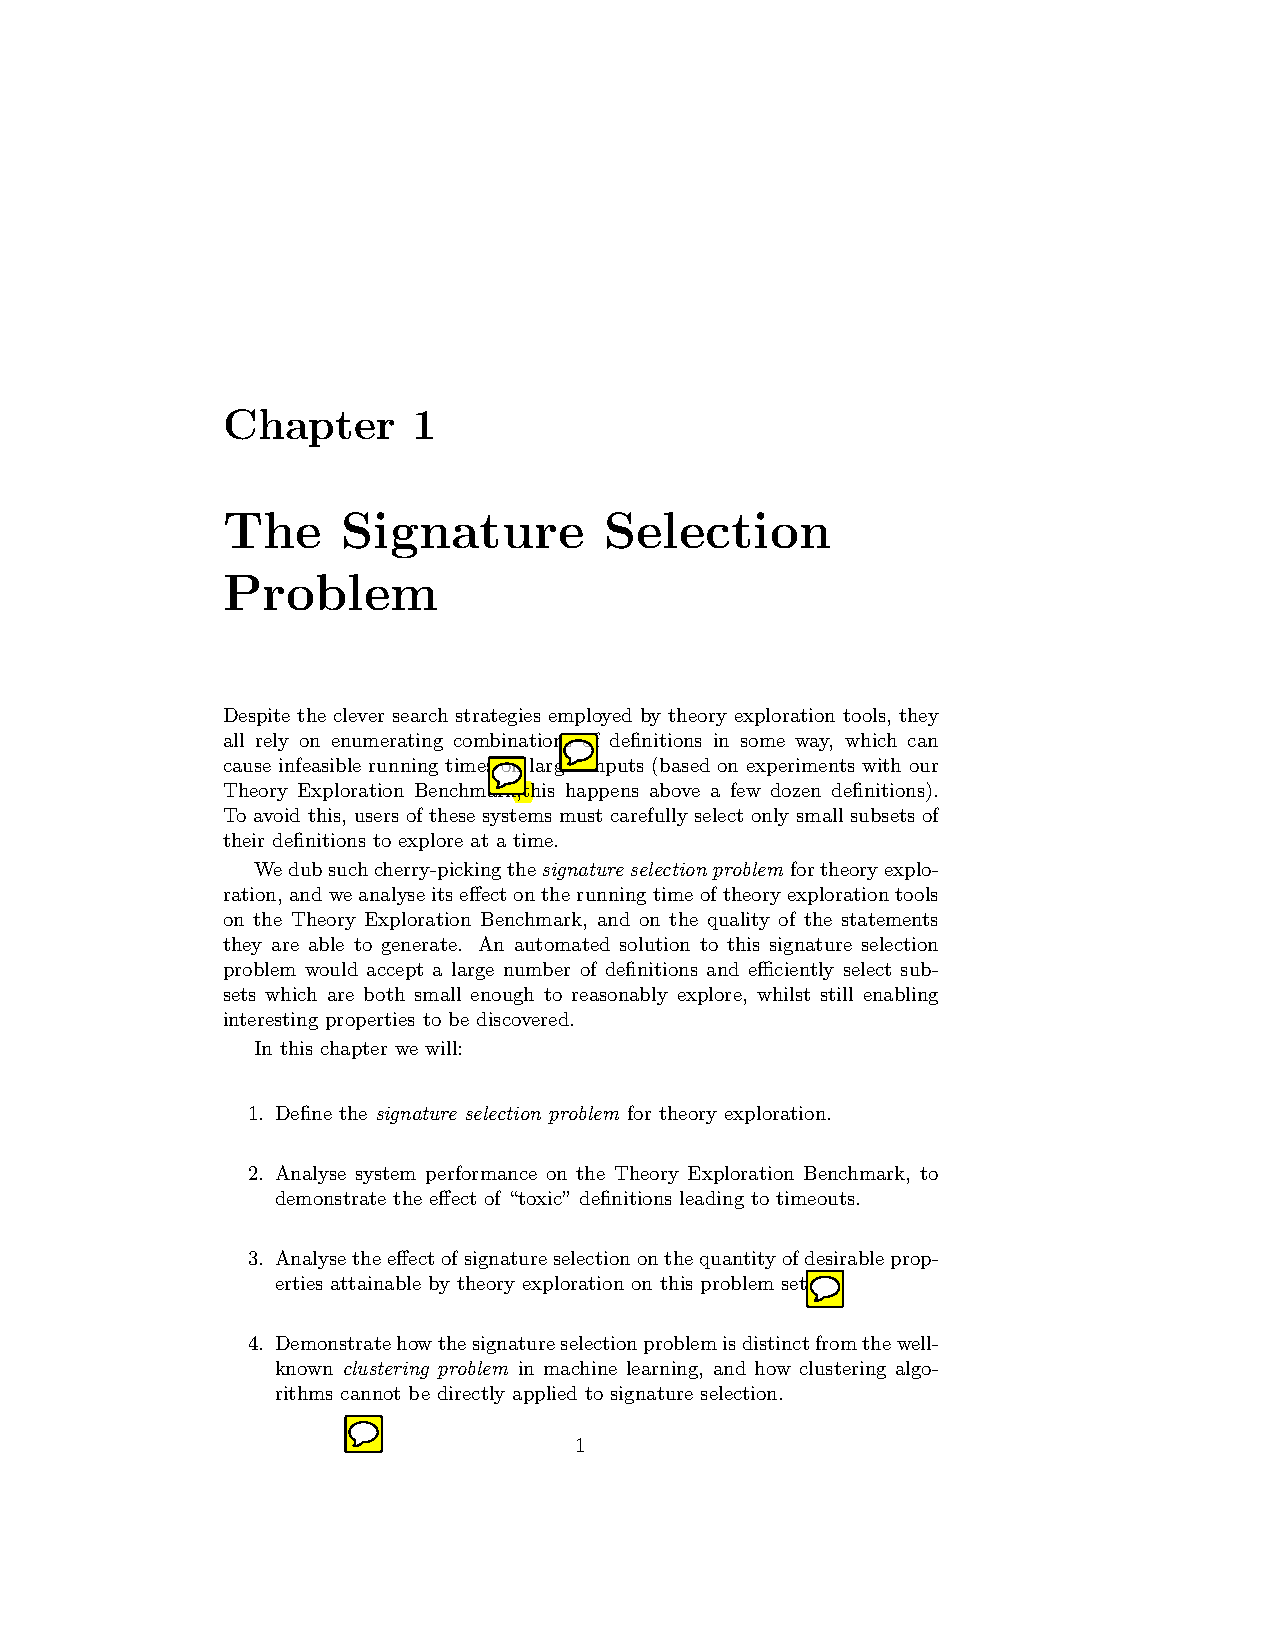
\includegraphics[width=\textwidth]{images/bucketing.png}
  \caption{Comparison of subset quality when selected by recurrent clustering
    (solid lines) versus pseudorandom selection (dashed lines). Darker lines
    show division into a greater number of subsets (between 1 and 20). The solid
    and dashed lines follow each other closely, indicating that clustering
    performs no better than random at signature selection.}
  \label{fig:bucketing}
\end{figure}

The signature selection problem is superficially similar to the
\emph{clustering} problem in machine learning: grouping data points based on
their similarity across multiple dimensions. To investigate this potential
relationship we created a signature selection method based on a \emph{recurrent
  clustering} algorithm for Haskell code: this flattens syntax trees into
vectors, substitutes fixed numbers for keywords and recurses to determine
suitable numbers for referenced expressions.

The results of this method are shown in Figure~\ref{fig:bucketing}, along with
the pseudorandom method as a control. The results of clustering turn out to be
no better than random; in fact the curves show surprisingly similar patterns.

\iffalse
% TODO
\section{Clustering}
\label{sec:clustering}

Our approach to scaling up \quickspec{} takes inspiration from two sources. The
first is relevance filtering, which makes expensive algorithms used in theorem
proving more practical by only considering clauses deemed ``relevant'' to the
problem~\cite{meng2009lightweight}.

Relevance is determined by comparing clauses to the target theorem, but theory
exploration does not have such a distinguished term. Instead, we are interested
in relationships between \emph{all} terms in a signature, and hence we need a
different algorithm for considering the relevance of \emph{all terms} to
\emph{all other terms}.

A natural fit for this task is \emph{clustering}, which attempts to group
similar inputs together in an unsupervised way. Based on their success in
discovering relationships and patterns between expressions in Coq and ACL2 (in
the ML4PG and ACL2(ml) tools respectively), we hypothesise that clustering
methods can fulfil the role of relevance filters for theory exploration:
intelligently breaking up large signatures into smaller ones more amenable to
brute force enumeration, such that related expressions are explored together.

Due to its use by ML4PG and ACL2(ml), we use \emph{k-means} clustering,
implemented in the Weka tool \cite{Holmes.Donkin.Witten:1994} by Lloyd's
algorithm \cite{lloyd1982least}, with randomly-selected input elements as the
initial clusters. Rather than relying on the user to provide the number of
clusters $k$, we use the ``rule of thumb'' given in
\cite[pp. 365]{mardia1979multivariate} of clustering $n$ data points into
$k = \lceil \sqrt{\frac{n}{2}} \rceil$ clusters.
\fi

%\section{Experiments}

% TODO: This was taken from the Background section, so probably doesn't fit here
% without some fiddling.
% TODO: Describe all of our experimental setups:
%
%  - The use of the TEBenchmark methodology for running QSpec, including the
%    sampling process
%
%  - Running our recurrent signature selection algorithm on samples from TEBenchmark,
%    including how we picked the sizes
%
%  - The definition of HashSpec and its use as control; how we ran all of the
%    same samples through it
%
%  - The use of optimal and pessimal oracles, defined via constraint
%    satisfaction. How we it was only feasible to run these up to size 10 (11?)

%We follow the tradition of prior practitioners and use an existing corpus of
%theorems as a \emph{ground truth} against which to compare results. To analyse
%behaviour on large inputs (i.e. those for which exploration is currently
%infeasible), as required to study the effects of signature selection, we have
%used the Theory Exploration Benchmark of section~\ref{sec:tebenchmark}, which is
%based on the Tons of Inductive Problems (TIP) problem set for theorem
%provers~\cite{claessen2015tip}.
